\documentclass[12pt]{article}
\usepackage[UTF8]{ctex}
\usepackage{amsmath,graphicx}
\usepackage[margin=1in]{geometry}
\usepackage{titlesec}
\usepackage{caption}
\usepackage{subcaption}
\usepackage{float}


\title{球形鸡在空气炸锅中的加热条件优化模型研究}
\author{刘泽睿\quad 李济坤\quad 刘厚振\quad 孙闫昊一}
\date{\today}

\begin{document}

\maketitle

\begin{abstract}
“外焦里嫩”是传统烤鸡理想的口感状态。本研究以球形鸡为简化模型,结合热传导、对流与辐射机制,建立空气炸锅加热过程中的热传递与水分迁移模型。通过引入临界焦化温度 $T_{crisp}$ 和安全食用温度 $T_{safe}$,结合时间控制,分析并优化炸鸡过程中温度与风速的动态变化规律,以实现表皮酥脆、内部多汁的理想加热效果。模型采用有限差分数值模拟方法,并通过灵敏度分析探讨参数变化对“外焦里嫩”实现的影响。研究结果可为空气炸锅等智能厨房设备提供理论支持与控制策略建议。
\end{abstract}

\section{引言}
“外焦里嫩”被广泛认为是烤鸡等高温熟食的理想状态,其中表皮需达到足够高温与干燥程度以实现焦脆感,而内部应保持在安全熟化温度下的多汁口感。随着空气炸锅等现代加热设备的发展,如何通过精准控制加热条件(如温度、风速、时间)以实现这一目标成为食品加工中的重要研究方向。

传统实验方法虽能获得经验性结果,但缺乏对内部传热过程的量化理解。为此,本研究将鸡肉简化为均质球体模型,尝试通过热传导与水分迁移方程建立完整数学模型,分析其加热过程中的温度场演化与水分流失特征,最终提出加热过程的优化策略。\cite{example}

\section{材料与方法}

\subsection{几何与物性假设}
大意:介绍建立的数学模型并对采用的假设和参数展开说明。 
\par 为便于数学建模,假设鸡肉为半径 $R$ 的均匀球体,具有统一的密度 $\rho$、比热容 $c$、热导率 $k$。空气炸锅加热腔内维持一定环境温度 $T_{env}(t)$,并产生速度为 $v(t)$ 的强迫对流。


\begin{figure}[htbp]
\centering
% \includegraphics[width=0.5\textwidth]{sphere_model.png}
\caption{球形鸡模型示意图与热交换机制}
\label{fig:model}
\end{figure}

\subsection{热传导模型}
大意:列出最基本的球形热传导方程,给出边界条件并求解
球体内部满足一维径向热传导方程:
\begin{equation}
\frac{\partial T}{\partial t} = \alpha \left( \frac{1}{r^2} \frac{\partial}{\partial r}\left(r^2 \frac{\partial T}{\partial r} \right) \right), \quad 0 < r < R
\label{eq:1}
\end{equation}
\par 其中\(\alpha = k/(\rho c)\)为热扩散率,$k$为热导率,\(\rho\)为密度,$c$为比热容。
\par 边界条件包括:
\begin{itemize}
\item 中心对称性:$\left.\frac{\partial T}{\partial r}\right|_{r=0} = 0$
\item 表面热交换(对流):
\begin{equation}
-k \left.\frac{\partial T}{\partial r}\right|_{r=R} = h(\left.T\right|_{r=R} - T_{env})
\end{equation}
\end{itemize}
\par 其中$h$是对流换热系数(又称表面传热系数)
% \par 求解得:\[ T(r, t)=T_{env}+\sum_{n=1}^{\infty} C_{n} \frac{\sin \left(\lambda_{n} r\right)}{r} e^{-\alpha \lambda_{n}^{2} t}\]
% \par 其中\[ C_n = \frac{2 (T_{0}-T_{env}) [\sin(\lambda_n R) - \lambda_n R \cos(\lambda_n R)]}{\lambda_n^2 R [1 - \cos(2\lambda_n R)/2]}\]

\subsection{水分迁移与蒸发模型}
在加热过程中,表皮水分不断蒸发形成干燥层,影响热阻与质构。假设水分主要由扩散与蒸发共同控制,建立如下方程:
\begin{equation}
\frac{\partial W}{\partial t} = D_w \nabla^2 W - R_{evap}(T, W)
\end{equation}
其中 $W$ 为含水率,$D_w$ 为水分扩散系数,$R_{evap}$ 为温度依赖型蒸发速率项。

\subsection{焦化与安全条件建模}

定义临界焦化温度 $T_{crisp} \approx 180^\circ$C,若表面温度达到并维持该值超过 $t_c$ 时间,则视为形成良好焦层。同时,内部温度需达到 $T_{safe} = 75^\circ$C 且不超过 $T_{dry} = 90^\circ$C 以避免肉质干柴。

\section{数值模拟与参数优化}
\subsection{热传导模型}
对方程带入不同的参数,画出温度随半径和时间变化的变化关系如图 2所示。
热传导方程为式\eqref{eq:1},将其代入半径分别为5cm、7.5cm、10cm的鸡块,使用python计算其分别在第5分钟、第10分钟、第20分钟时的温度分布如图\ref{fig:chicken}所示。
\begin{figure}[htbp]
	\begin{minipage}{0.32\linewidth}
		\vspace{3pt}
		\centerline{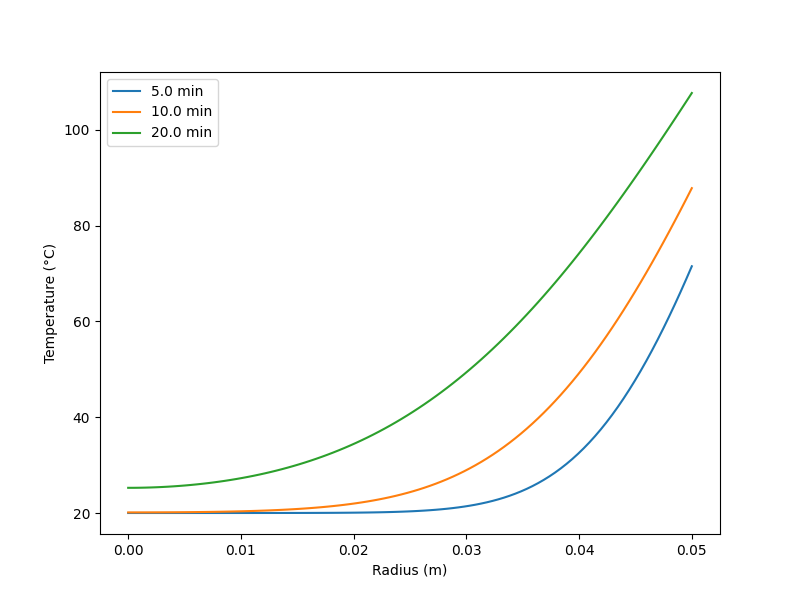
\includegraphics[width=\textwidth]{heat_distribution1.png}}
		\centerline{r=5cm}
	\end{minipage}
	\begin{minipage}{0.32\linewidth}
		\vspace{3pt}
		\centerline{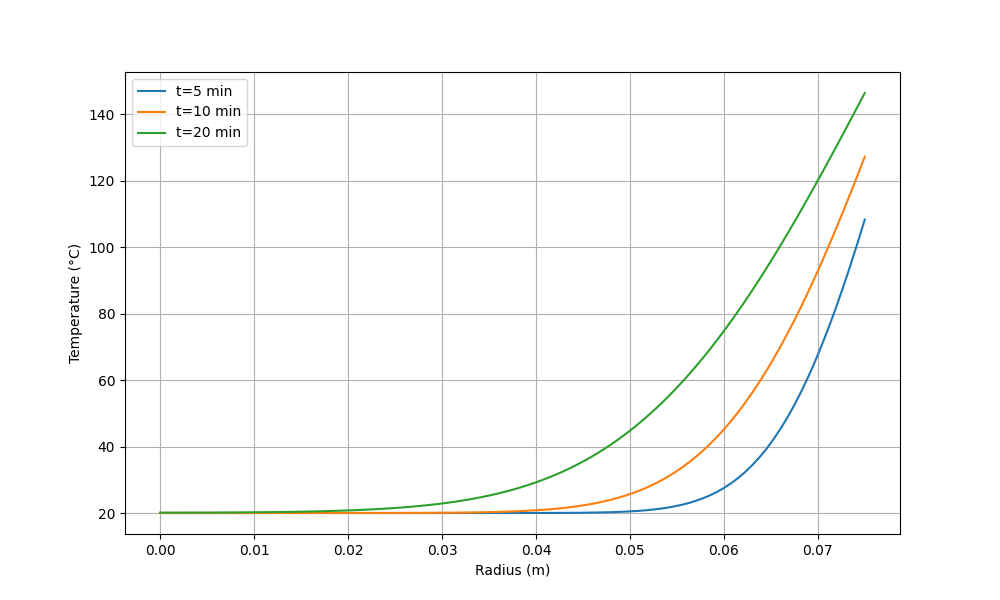
\includegraphics[width=\textwidth]{heat_distribution2.png}}
		\centerline{r=7.5cm}
	\end{minipage}
	\begin{minipage}{0.32\linewidth}
		\vspace{3pt}
		\centerline{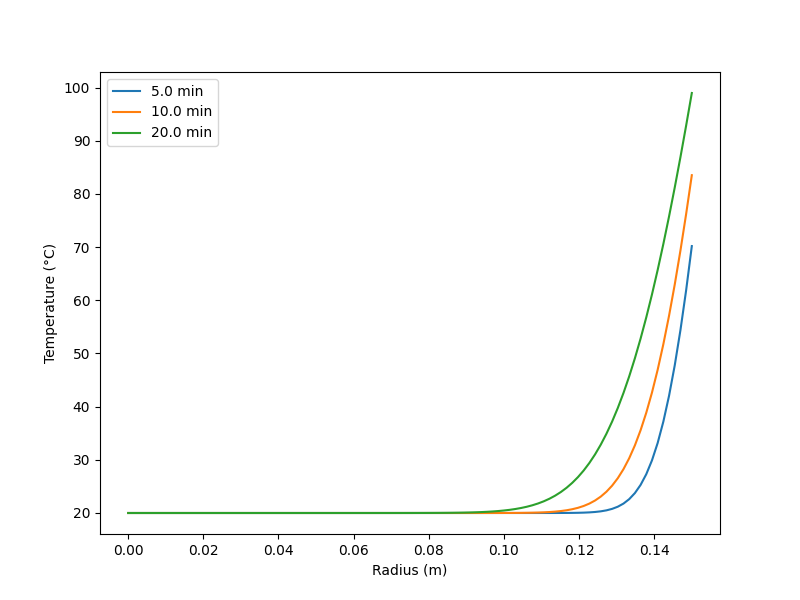
\includegraphics[width=\textwidth]{heat_distribution3.png}}
		\centerline{r=10cm}
	\end{minipage}
	\caption{球形鸡模型温度随半径和时间变化理论计算结果示意图}
	\label{fig:chicken}
\end{figure}

\subsection{水分迁移与蒸发模型}
采用显式有限差分法对传热与水分迁移方程进行数值求解。初始条件设鸡体温度为 $T_0 = 20^\circ$C,含水率 $W_0 = 0.7$。

\begin{figure}[htbp]
\centering
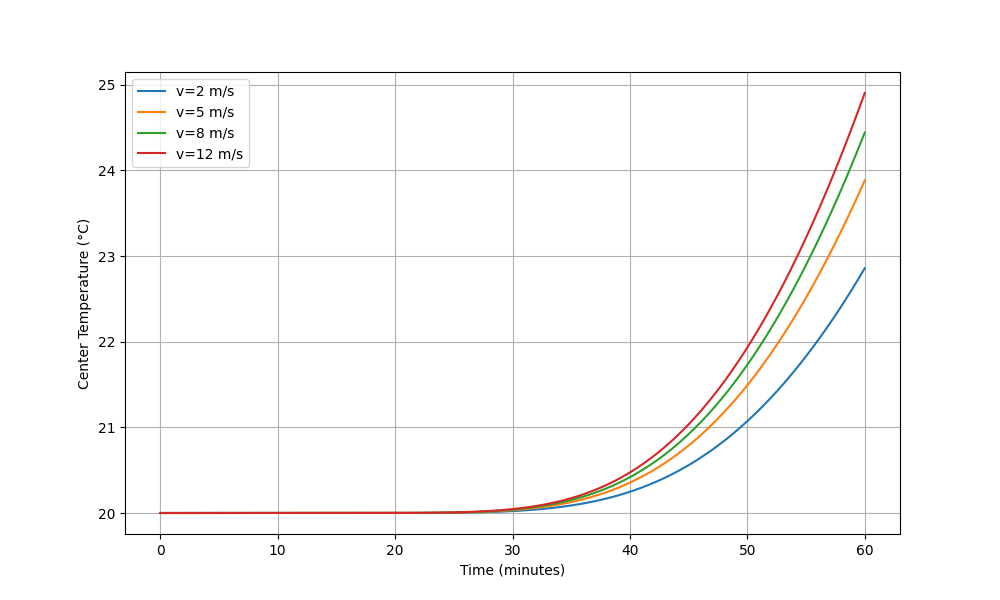
\includegraphics[width=0.8\textwidth]{wind.jpg}
\caption{不同风速条件下鸡肉温度随时间的演化}
\end{figure}

通过调整空气炸锅的风速 $v(t)$ 与炉温 $T_{env}(t)$,探索使表面温度迅速达到 $T_{crisp}$ 而内部缓慢升温至 $T_{safe}$ 的最优策略。

\begin{figure}[htbp]
\centering
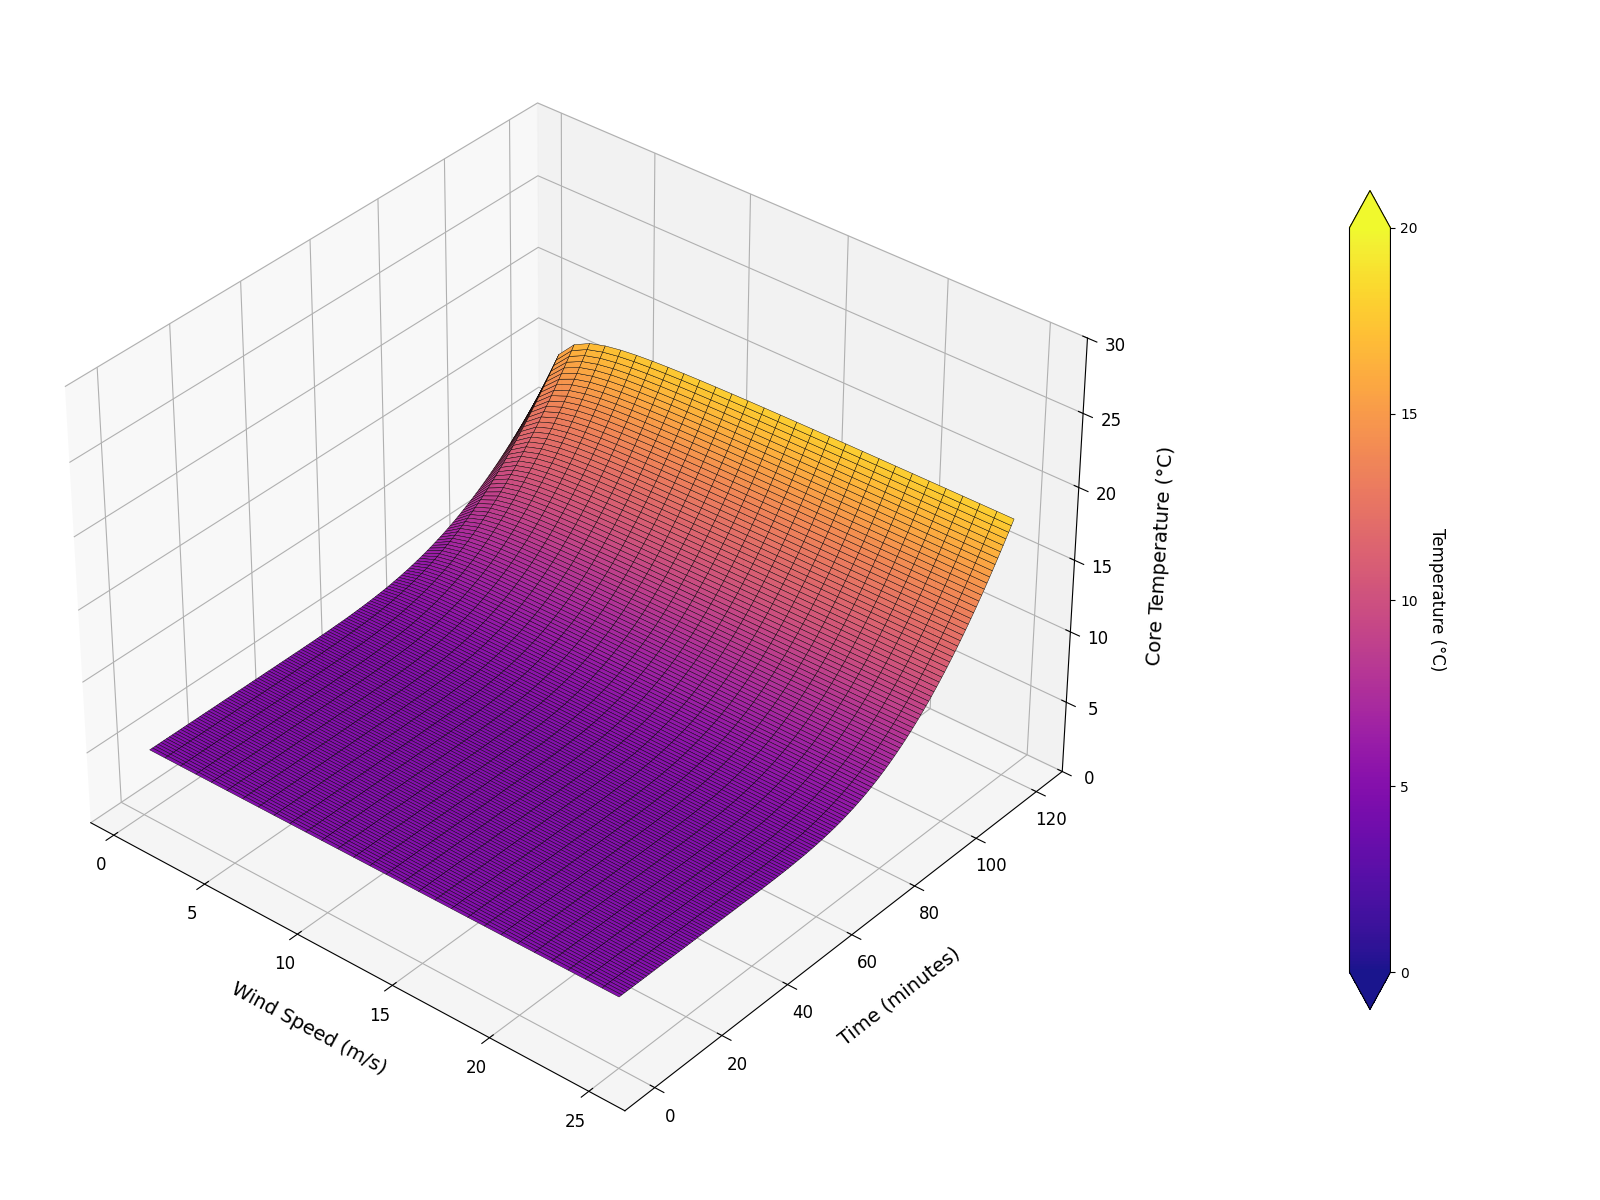
\includegraphics[width=0.8\textwidth]{3d.png}
\caption{温度-风速-时间三维响应面图}
\end{figure}

\section{结果与分析}
仿真结果显示:
\begin{itemize}
\item 风速增加有助于加快表皮升温,但内部温度上升较慢,利于“外焦里嫩”。
\item 温度过高或维持过久易导致内部干燥,需设定分段温控策略。
\item 水分蒸发主要集中在 $r \in [0.9R, R]$ 区域,对应焦化层形成部位。
\end{itemize}

\begin{figure}[htbp]
\centering
% \includegraphics[width=0.6\textwidth]{moisture_layer.png}
\caption{表层含水率随时间变化,显示焦化区演化}
\end{figure}

\section{讨论}
本模型通过合理简化提供了一个分析空气炸锅加热鸡肉过程的基础框架。虽然未考虑鸡体结构非均质性(如骨骼、皮层差异),但模型足以揭示“外焦里嫩”实现的主要机制。未来可拓展至不规则形状建模、实验验证及机器视觉结合。

\section{结论}
本研究建立了空气炸锅中球形鸡加热过程的耦合热-湿模型,并通过数值模拟优化了加热策略。结果表明,适当控制风速与温度的变化可有效实现表焦内嫩的目标。该研究为智能厨房设备中的热控算法设计提供了理论依据。

\section*{致谢}
感谢指导教师在模型设定与数值模拟方面的悉心指导,以及实验数据的支持。

\bibliographystyle{plain}
\bibliography{references.bib}

\end{document}
